\documentclass[11pt,a4paper]{article}
\usepackage[utf8]{inputenc}
\usepackage[spanish]{babel}
\usepackage{amsmath}
\usepackage{amsfonts}
\usepackage{amssymb}
\usepackage{makeidx}
\usepackage{graphicx}
\usepackage{lmodern}
\usepackage{kpfonts}
\usepackage{parskip}
\usepackage[left=2cm,right=2cm,top=2cm,bottom=2cm]{geometry}
\author{Miguel Angel Xamie Diaz Fuentes}
\begin{document}
\begin{center}
\begin{LARGE}
\textbf{INGENIERÍA MECATRÓNICA}\\
\end{LARGE}
{\large Sistemas Eletrónicos De Interfaz}\\

\begin{figure}[hbtp]
\centering

\includegraphics[scale=0.80]{UPZMG_Mecatr_nica.png}
\end{figure} 

\begin{center}
\begin{LARGE}
EV-3-1 DIAGRAMA ELÉCTRICO DE LA INTERFAZ DE POTENCIA - PRACTICA 9
\end{LARGE}
\end{center}

\begin{Large}
\textbf{Alumno}
\\\textit{Miguel Angel Xamie Diaz Fuentes\\Raul Jimenez Cortez}
\textbf{\\Maestro}
\\\textit{Morán Garabito Carlos Enrique}
\textbf{\\Fecha de Entrega}
\\\textit{08/11/2019}
\textbf{\\Grupo}
\\\textit{4-B}\\
\textbf{Período Cuatrimestral}\\
\textit{2019-Septiembre-Diciembre}
\\
\end{Large}

\end{center}

\footnote{Universidad Politécnica De La Zona Metropolitana De Guadalajara} 

\newpage

\section{Marco Teórico}


Las interfaces de potencia son dispositivos intermedios entre nuestro microcontrolador y aquellos aparatos que requieran cantidades de corriente mayores a los que pueden manejar nuestro microcontrolador (por lo general estamos hablando de 40 miliamperios como máximo por pin), motores de paso, motores DC, servo motores, lamparas incandescentes, reflectores, grupos de leds son ejemplos de dispositivos que podríamos a llegar a controlar desde el microcontrolador a través de las interfaces de potencia, es un grave error tratar de conectarlos directamente a los pines del microcontrolador. Nos valdremos de transistores, reles, puentes-H o interfaces eléctronicas de control, para construir nuestras interfaces de potencia.

\textbf{Transistores:}

Los transistores pueden funcionar como amplificadores o interruptores, si los utilizamos como interruptores al igual que los relés pueden manejar corrientes altas, controlados por corrientes bajas. Los transistores son dispositivos de tres terminales (patas) y en el caso de los transistores bipolares sus terminales se llaman emisor base y colector, al poner una corriente pequeña en la base, una corriente alta puede pasar del colector al emisor. Entre los transistores bipolares podemos diferenciar dos tipos NPN y PNP.

\textbf{MOSFET:}

Los MOSFET también son para circuitos de conmutación de potencia. A diferencia de los transistores de unión bipolar (BJT), el tipo de transistor de potencia de la competencia, los MOSFET no requieren un flujo continuo de corriente de accionamiento para permanecer en el estado ON. Además, los MOSFET pueden ofrecer velocidades de conmutación más altas, pérdidas de potencia de conmutación más bajas, resistencias de encendido más bajas y una susceptibilidad reducida a la fuga térmica. En las fuentes de alimentación de modo conmutado (SMPS), los MOSFETS se utilizan a menudo como elementos de conmutación, así como para la corrección del factor de potencia (PFC).

\textbf{TIP41C:}

El TIP41C es un transistor de potencia de plástico diseñado para usarse en aplicaciones de amplificación y conmutación de propósito general. 

\begin{itemize}
\item Complemento del TIP42C. 
\item Tiempo de encendido de 0.6us.
\item Tiempo de apagado de 1.4us.
\item Aplicaciones: Audio, Industrial, Procesado de Señal.
\end{itemize}

\textit{Descripción del transistor}

\begin{itemize}
\item Polaridad del transistor: NPN.
\item Voltaje colector-emisor  V (br) ceo: 100 V.
\item Voltaje colector base VCBO: 100 V.
\item Voltaje emisor base VEBO: 5 V.
\item Disipación de potencia Pd: 65 W.
\item Corriente continua colector DC: 6 A.
\item Corriente pico: 10 A.

\footnote{Universidad Politécnica De La Zona Metropolitana De Guadalajara} 

\newpage

\item Ganancia de corriente continua hFE: 75.
\item Frecuencia de transición ft: 3 MHz.
\item Temperatura de operación mínima: -65 °C.
\item Temperatura de operación máxima: 150 °C.
\item  Encapsulado: TO-220
\end{itemize}

\section{Desarrollo}

\subsection{Practica 9 (Diagrama A - Convertidor BUCK DC-DC)}

El convertidor reductor es un tipo muy simple de convertidor CC-CC que produce un voltaje de salida que es menor que su entrada. El convertidor reductor se llama así porque el inductor siempre *contradice* o actúa contra el voltaje de entrada. La tensión de salida de un convertidor reductor ideal es igual al producto del ciclo de trabajo de conmutación y la tensión de alimentación.

\begin{figure}[hbtp]
\centering
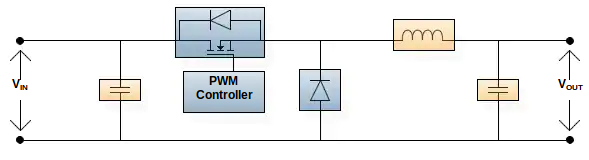
\includegraphics[scale=0.80]{1.png}
\end{figure} 

\textbf{\textit{PWM 555}}


Este circuito integrado se utiliza para activar o desactivar circuitos durante intervalos de tiempo determinados, es decir se usa como temporizador. Para ello, lo combinaremos con otros componentes cuyas características y forma de conexión en el circuito, determinarán la duración de los intervalos de tiempo del 555, y si estos intervalos se repitan continuamente o no.


\begin{figure}[hbtp]
\centering
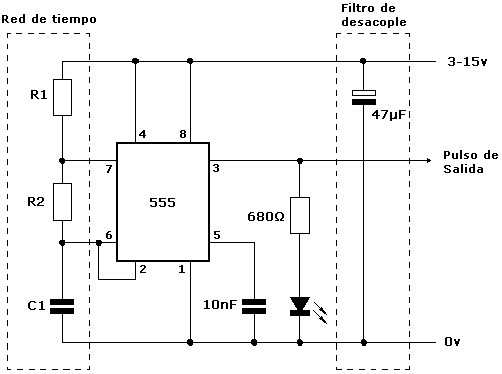
\includegraphics[scale=0.50]{2.png}
\end{figure} 

\footnote{Universidad Politécnica De La Zona Metropolitana De Guadalajara} 

\newpage

Una vez armado la señal de pulso de puede apreciar de esta forma:

\begin{figure}[hbtp]
\centering
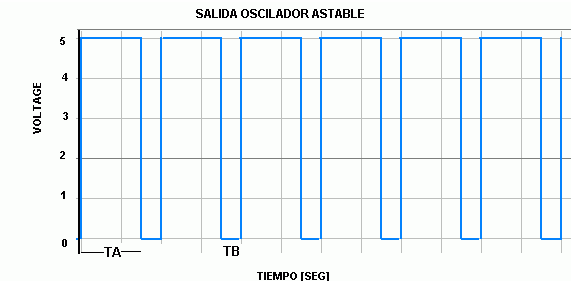
\includegraphics[scale=0.50]{3.png}
\end{figure} 

Con esta señal la interfaz del buck se debe alimentar para que el convertidor mantenga su corriente con el voltaje reducido y que alimente los leds. La función del mosfet es mantener la carga que guardan los capacitores y que también la bobina no haga un incremento de corriente esto con la función del diodo dentro del mosfet. Se debe mantener con cuidado la temperatura del mosfet ya que incremente bastante en poco tiempo, y tener cuidado de no realizar conexiones inversas ya que pueden explotar los capacitores.

\textbf{Estado ON Convertidor}

\begin{figure}[hbtp]
\centering
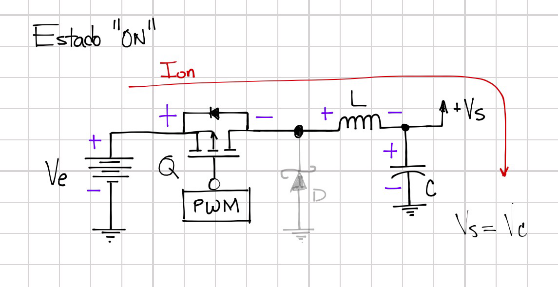
\includegraphics[scale=0.50]{ON.png}
\end{figure} 

Cuando el transistor conduce, la corriente va desde la fuente de entrada hasta el capacitor, cargando a su paso la bobina. La ecuación, siguiendo las leyes de kirchhoff, queda: $ V_c = V_{Qm} + V_{Lon} + V_s $.


El diodo, como se puede apreciar, no conduce, ya que en ese momento esta polarizado inversamente. En este estado, denominado comúnmente en los libros como *estado ON* la función del circuito es cargar la bobina, nuestro principal elemento de almacenamiento de energía, además de  de alimentar el circuito de carga con el voltaje suficiente por medio del capacitor.


\footnote{Universidad Politécnica De La Zona Metropolitana De Guadalajara} 

\newpage

\textbf{Estado OFF  Convertidor}

\begin{figure}[hbtp]
\centering
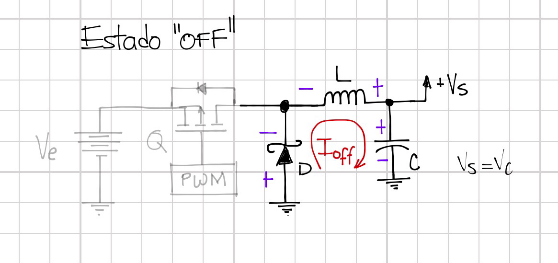
\includegraphics[scale=0.50]{OFF.png}
\end{figure} 

Cuando el transistor se pone en un estado de corte, es decir, no hay conducción, la fuente principal de energía no alimenta el circuito. En ese momento se aprovecha la energía del inductor, almacenada en forma de campo magnético, para hacer circular una corriente por el circuito. Esta corriente sigue alimentando al capacitor y mantiene el nivel de voltaje a la salida. La ecuación para este *estado OFF* queda: $ - V_D = - V_{Loff} + V_s $

Ahora bien, entre estos dos estados, de conducción y no conducción es como se transforma el voltaje de entrada al de salida. Al conmutar entre estados, a una frecuencia fija, la conversión dependerá de de cuanto dura cada estado con respecto a la frecuencia. Por convención usaremos el estado de conducción como base, será nuestro ciclo de trabajo. Por lo tanto usaremos para conmutar el transistor un circuito oscilador en el que podamos cambiar su ciclo de trabajo, es decir un circuito de oscilación pwm.

\begin{figure}[hbtp]
\centering
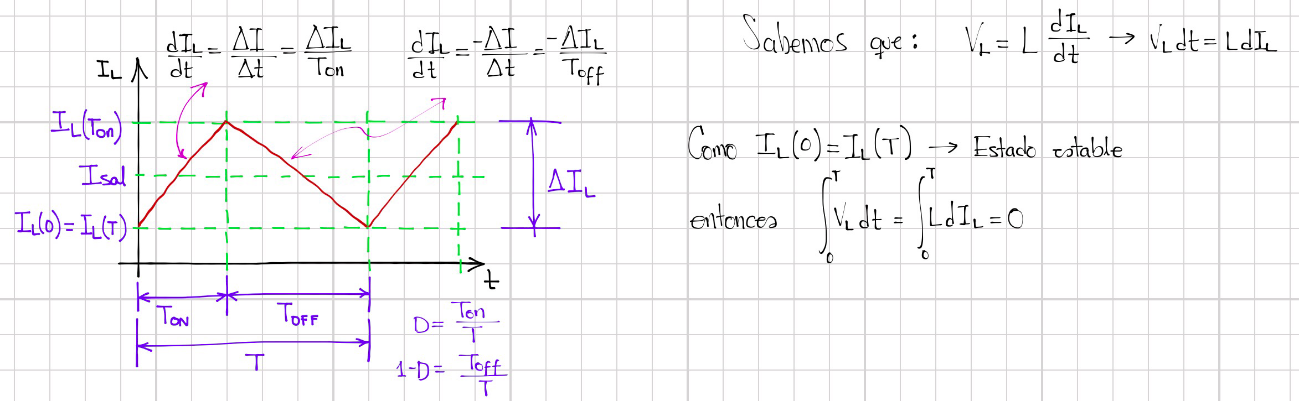
\includegraphics[scale=0.35]{4.png}
\end{figure}

\footnote{Universidad Politécnica De La Zona Metropolitana De Guadalajara} 

\newpage

\section{Evidencias}

\begin{figure}[hbtp]
\centering
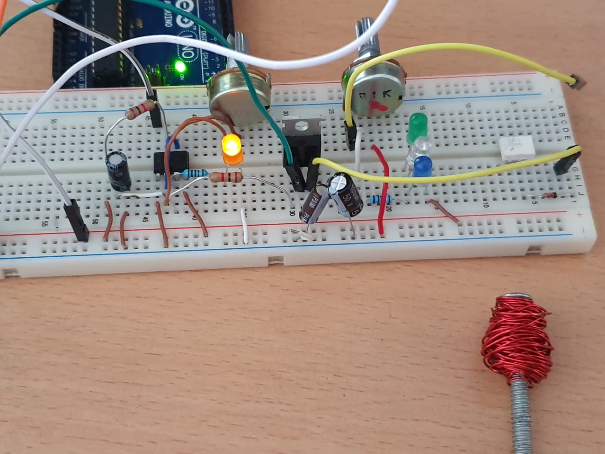
\includegraphics[scale=0.80]{5.png}
\end{figure}

\section{Practica 9 (Diagrama C TIP41C)}

En este circuito la función era amplificar una señal a tal punto que podamos encender 3 emisores de luz o led's los, para esto se utilizo un entrada de 1.5v la cual pasarían por bobinas que hacen que por el cable circula una corriente tiene a su alrededor un campo magnético, siendo el sentido de flujo del campo magnético, el que establece la ley de la mano derecha.
Al estar el inductor hecho de espiras de cable, el campo magnético circula por el centro del inductor y cierra su camino por su parte exterior. Una característica interesante de los inductores es que se oponen a los cambios bruscos de la corriente que circula por ellas.

Esto significa que a la hora de modificar la corriente que circula por ellos (ejemplo: ser conectada y desconectada a una fuente de alimentación de corriente continua), esta intentará mantener su condición anterior.

Este caso se da en forma continua, cuando una bobina esta conectada a una fuente de corriente alterna y causa un desfase entre el voltaje que se le aplica y la corriente que circula por ella. 

\footnote{Universidad Politécnica De La Zona Metropolitana De Guadalajara} 

\newpage

Entonces cuando tenemos este voltaje de entrada de 1.5v se carga el capacitar haciendo que la base se active cuando esta se carga y permite el paso de la corriente por el emisor y el colectar también la bobina conectada con los leds en serie permite que aumente la corriente en conjunto con la carga de los capacitores. Lo cual nos permite observar la amplificación de señal y tipos de circuitos que se realizan con estos materiales muy comunes a continuación se puede ver las evidencias de la practica encendido y apagado.

\section{Evidencias}

\begin{figure}[hbtp]
\centering
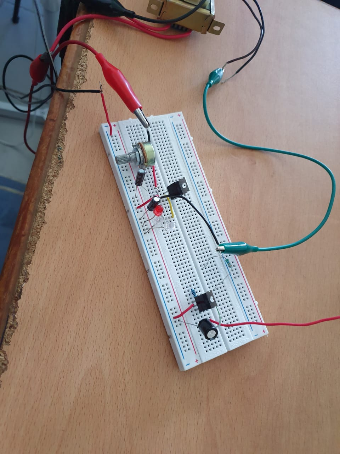
\includegraphics[scale=0.50]{6.png}
\end{figure}
\begin{figure}[hbtp]
\centering
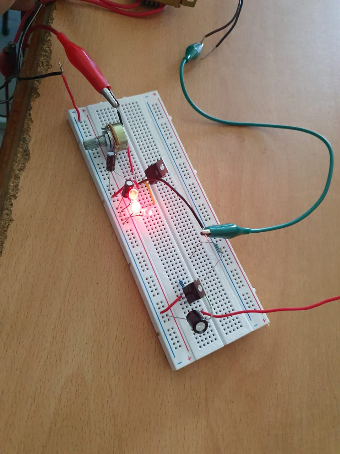
\includegraphics[scale=0.50]{7.png}
\end{figure}

\footnote{Universidad Politécnica De La Zona Metropolitana De Guadalajara} 

\newpage

\section{Conclusiones}

La competencia aprendida en esta practica fue como se crean interfaces de potencia con componentes ya utilizados en practicas anteriores las cuales con actuadores como relevadores o en este caso transistores activan otras potencias que permiten funcionar un circuito o actuadores dependiendo los circuitos que se realicen todo esto da una idea de como la potencia es esencial para poder funcionar un circuito ya que el consumo del mismo o algún calculo mal provoca que no funciona adecuadamente. Así que con el convertidor buck observamos la potencia de los leds activados por un pulso y por el tip podemos observar con la carga del capacitor activando la base permite el paso de la corriente cargada con una bobina y un capacitor y encienda unos los emisores de luz. 

\bibliography{Referencia}
\begin{thebibliography}{X}

\bibitem{Baz} \textsc{THE DECCA DIGITAL.} \textit{Electrónica de  potencia.}Multiplexación.

\bibitem{Baz} \textsc{MANCINI, GINO.} \textit{Modulación por impulsos codificados.} 
Mastering System (2007).

\bibitem{Baz} \textsc{HODGES, DAVID A. (1999).} \textit{Darlintong's - Contributions To Transistor Circuit Desing.} 
IEEE Transactions on Circuits and Systems-I: Fundamental Theory and Applications.

\bibitem{Baz} \textsc{HOROWITZ, PAUL; WINFIELD HILL (1989).} \textit{The Art of electronics.} 
Cambridge University Press. ISBN 0-521-37095-7.


\end{thebibliography}

\bibliographystyle{plain}




\end{document}